\section{What is PYro?}
PYro is a flexible platform for conveniently working with gobs and gobs of thermodynamic data in scripts and at the command line in Python.  The intent behind PYro is probably best described with an apocryphal story.

\begin{verse}
There once was a student\\
with work ethic prudent\\
she scripted to speed her work.

In Python t'was coded,\\
so when it was loaded,\\
she could all the tedium shirk.

A thermodynamic\\
fluid mechanic\\
problem she had solved.

Her colleagues were avid\\
she share the package\\
frustration to resolve.

Good, was the mood.\\
Researchers all cooed,\\
until she read her mail.

With no contradiction,\\
viscosity-friction;\\
with it her package would sail.

She furiously typed\\
new modules to write.\\
The people, they must be heard.

What thanks had it gotten?\\
why, STEAM she'd forgotten!\\
Without it, the code was absurd.

Downtrodden indeed,\\
she sat at the screen,\\
multiphase soon to add.

Though coffee was drunk\\
and sleepless nights sunk,\\
her code, it really was bad!

The syntax was rambling\\
no hope of unscrambling\\
the endless nonsensical edits.

Compatible, reverse,\\
a programmer's curse\\
no fixing - it's time to shred it.

``I'm done,'' she then plead.\\
To the airport, she fled.\\
``I'll fly off to someplace that's random.''

Her useful creation\\
was once a sensation;\\
forgotten and now is abandoned.

Her colleagues still moan,\\
``Please pick up your phone!\\
Your software, it just isn't working.''

Ye coders beware\\
the fate most unfair,\\
within all your projects is lurking.
\end{verse}

With a flexible framework that allows users to define their own data and even their own classes, the hope is that over time PYro will graudally be extended to do the jobs that people need most, but in a way that is ``Pythonic'' and extensible.  In that way, PYro is distinguished from other excellent thermodynamic resources (like Cantera) by its emphasis on being application agnostic.  

PYro is easily installed using a standard setup script, convenient to use from the command line, but also highly configurable.  To get a feel for how easy PYro is to use, look at section \ref{sec:start}.

\underline{What can PYro do?}  The PYro classes supply methods for calculating most common thermodynamic properties from temperature and pressure such as density, enthalpy, entropy, internal energy, molecular weight, specific heats, specific heat ratio, and specific volume.

While version 1.1 included only ideal gas data, version 1.2 includes properties of water and steam.  There are plans to include refrigerants in later releases.

The addition of the psolve() function to all classes makes property inversion possible.  In other words, it is possible to determine the pressure and temperature at which a substance will have a given entropy and enthalpy.  This comes in handy for cycle analysis and flame temperature calculations.

\underline{What can't PYro do?}  In addition to many others, all of the species supported by the \href{http://combustion.berkeley.edu/gri-mech/}{GRIMech reaction database} are included, but the corresponding chemical kinetic data are not.  While this could possibly change one day, \href{http://cantera.github.io/docs/sphinx/html/index.html}{Cantera} already offers excellent chemical kinetics support, so adding this functionality is not a priority.  This is an example where Cantera is probably just a better tool for the job than PYro.

It is also worth noting here that psolve() is not as robust as it should be for steam in the vicinity of phase changes.  The abrupt discontinuity in properties causes problems for the Newton algorithim or which psolve is built.  This will definitely be addressed in the future.

\section{Getting Started}\label{sec:start}
Whether you are just getting started or you are curious whether PYro will work for your application, this section should be what you need.

First, we begin with a bit of preparation.
\begin{verbatim}
>>> import pyro
>>> import matplotlib.pyplot as plt
>>> import numpy as np
\end{verbatim}

It can be very simple to get some quick information.
\begin{verbatim}
>>> O2 = pyro.get('O2')
>>> O2.cp(T=432)
0.95049900128261733
\end{verbatim}

It can be very simple to get lots of quick information.
\begin{verbatim}
>>> T = np.arange(300,4000,10)
>>> plt.plot(T, O2.h(T))
>>> plt.xlabel('Temperature (K)');plt.ylabel('Enthalpy (kJ/kg)')
>>> plt.grid('on')
\end{verbatim}

\begin{figure}[h!]
\begin{center}
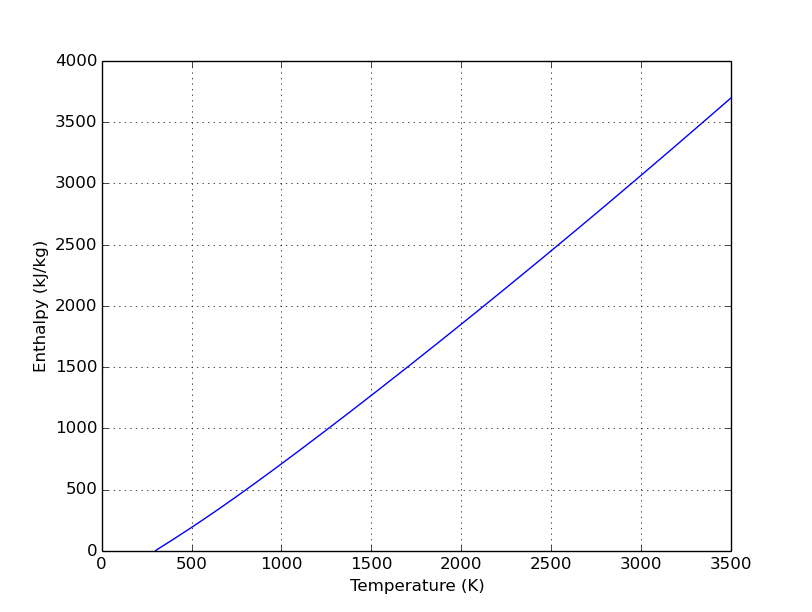
\includegraphics[width=.75\linewidth]{fig/o2h}
\caption{Enthalpy of diatomic oxygen.}
\end{center}
\end{figure}

Methods are available to calculate a number of common thermodynamic quantities; density (\verb|.d|), enthalpy (\verb|.h|), entropy (\verb|.s|), internal energy (\verb|.e|), molecular weight (\verb|.mw|), specific heats (\verb|.cp| and \verb|.cv|), specific heat ratio (\verb|.k|), and others.

Data are available for mixtures too.  In addition to the typical methods for calculating properties, the \verb|mixture| class provides methods to interrogate the mass, molar, and fractional mass and molar contents.
\begin{verbatim}
>>> air = pyro.get('air')
>>> air.M()
{u'N2': 21.88, u'Ar': 0.373, u'CO2': 0.013, u'O2': 6.704}
>>> air.N()
{u'N2': 0.7810547809262709, u'Ar': 0.009337138279763693, 
u'CO2': 0.00029539076790238467, u'O2': 0.20950785654462042}
>>> air.Y()
{u'N2': 0.7552640662754573, u'Ar': 0.012875388332758024, 
u'CO2': 0.0004487400759406282, u'O2': 0.23141180531584396}
>>> air.X()
{u'N2': 0.780902374928423, u'Ar': 0.009335316338574262, 
u'CO2': 0.0002953331287638292, u'O2': 0.20946697560423902}
>>> air.d( T=400, P=2.0 )
1.741805229300913
\end{verbatim}

The \verb|info()| function prints a summary of all available species.
\begin{verbatim}
>>> pyro.info()
  PYro
Thermodynamic computational tools for Python
version: 1.2
-------------------------------
ID      Modified    Type
-------------------------------
Ar      4/7/2016    igfit
Ar+     4/7/2016    igtab
Ar2     4/7/2016    igtab
C       4/7/2016    igfit
C2H     4/7/2016    igfit
C2H2    4/7/2016    igfit
C2H3    4/7/2016    igfit
C2H4    4/7/2016    igfit
C2H5    4/7/2016    igfit
C2H6    4/7/2016    igfit
C3H7    4/7/2016    igfit
C3H8    4/7/2016    igfit
CH      4/7/2016    igfit
CH2     4/7/2016    igfit
CH2(S)  4/7/2016    igfit
-------------------------------
ID      Modified    Type
-------------------------------
CH2CHO  4/7/2016    igfit
CH2CO   4/7/2016    igfit
CH2O    4/7/2016    igfit
CH2OH   4/7/2016    igfit
CH3     4/7/2016    igfit
CH3CHO  4/7/2016    igfit
CH3O    4/7/2016    igfit
CH3OH   4/7/2016    igfit
CH4     4/7/2016    igfit
CN      4/7/2016    igfit
CO      4/7/2016    igfit
CO2     4/7/2016    igfit
Cl      4/7/2016    igtab
F       4/7/2016    igtab
F2      4/7/2016    igtab
-------------------------------
ID      Modified    Type
-------------------------------
F5      11/6/2015   mixture
FK      4/7/2016    igtab
FN      4/7/2016    igtab
FO      4/7/2016    igtab
H       4/7/2016    igfit
H2      4/7/2016    igfit
H2CN    4/7/2016    igfit
H2O     4/7/2016    igfit
H2O2    4/7/2016    igfit
H35     11/6/2015   mixture
HCCO    4/7/2016    igfit
HCCOH   4/7/2016    igfit
HCN     4/7/2016    igfit
HCNN    4/7/2016    igfit
HCNO    4/7/2016    igfit
-------------------------------
ID      Modified    Type
-------------------------------
HCO     4/7/2016    igfit
HNCO    4/7/2016    igfit
HNO     4/7/2016    igfit
HO2     4/7/2016    igfit
HOCN    4/7/2016    igfit
He      4/7/2016    igtab
He+     4/7/2016    igtab
I       4/7/2016    igtab
I2      4/7/2016    igtab
IK      4/7/2016    igtab
Kr      4/7/2016    igtab
N       4/7/2016    igfit
N2      4/7/2016    igfit
N2O     4/7/2016    igfit
NCO     4/7/2016    igfit
-------------------------------
ID      Modified    Type
-------------------------------
NH      4/7/2016    igfit
NH2     4/7/2016    igfit
NH3     4/7/2016    igfit
NNH     4/7/2016    igfit
NO      4/7/2016    igfit
NO2     4/7/2016    igfit
Ne      4/7/2016    igtab
Ne+     4/7/2016    igtab
O       4/7/2016    igfit
O2      4/7/2016    igfit
OH      4/7/2016    igfit
Rn      4/7/2016    igtab
S       4/7/2016    igtab
S2      4/7/2016    igtab
S3      4/7/2016    igtab
-------------------------------
ID      Modified    Type
-------------------------------
S4      4/7/2016    igtab
Xe      4/7/2016    igtab
air     11/6/2015   mixture
steam   12/24/2015  if97
\end{verbatim}

When called with the name of a species, it returns more specific information information. 
\begin{verbatim}
>>> pyro.info('HCO')
***
Information summary for substance: "HCO"
***
Uses class:   igfit

Loaded from:  C:\Users\crm28\WinPython-64bit-2.7.10.2\python-2.7.10.amd64\lib\site-packages\pyro\data\HCO.hpd

Last updated: 10:07 December 5, 2015

These data are adapted from the GRI-Mech website,
http://www.me.berkeley.edu/gri-mech/
and are credited to
B.J. McBride, S. Gordon, and M.A. Reno, 'Coefficients for Calculating
Thermodynamic and Transport Properties of Individual Species', NASA Report
TM-4513, October 1993
A. Burcat and B. McBride, '1994 Ideal Gas Thermodynamic Data for
Combustion and Air- Pollution Use', Technion Report TAE 697, December 1993
Adaptation by Chris Martin (c)2015.
Units are supplied in: energy kJ temperature K mass kg molar kmol

>>>  pyro.info('air')
***
Information summary for substance: "air"
***
Uses class:   mixture

Loaded from:  C:\Users\crm28\WinPython-64bit-2.7.10.2\python-2.7.10.amd64\lib\site-packages\pyro\data\air.hpd

Last updated: 10:34 December 5, 2015

The composition of air is taken from section 14 page 20 of the the CRC
Handbook of Chemistry and Physics 96th ed, 2015-2016.
www.hbcpnetbase.com
Trace gases (those present in less than 0.01% by volume) are neglected, as
they will not contribute substantially to the thermodynamic properties.
Original work is credited to:
COESA, "U.S. Standard Atmosphere, 1976", U.S. Government Printer Office,
Washington D.C., 1976.
Adapted by Chris Martin (c) 2015.
\end{verbatim}


\section{Installation}
Installation is accomplished through the \verb|setup.py| script in the root directory of the package distribution.  The following steps should produce a working installation of PYro.
\begin{enumerate}
\item Extract the package\\
\texttt{tar -xjvf \lpackage}
\item Execute the setup script\\
\texttt{cd \package}\\
\texttt{python setup.py install}\\
\end{enumerate}

On a Windows installation, the package will appear as a zip file, \texttt{\wpackage{}}, instead of a compressed tarball.  Right-click on the file and select ``Extract All'' to unzip the file.  That should create the \texttt{\package} folder, wherein lies the setup file.  From within a command prompt, navigate to the directory and execute the setup file.
\begin{verbatim}
cd C:\path\to\package
python.exe setup.py install
\end{verbatim}

On a Linux installation, you may need to use \verb|sudo| to execute the setup script if you don't have write privileges to the Python installation directory.

\subsection{Linux Maual Installation}
If you want to perform an unconventional installation, you will need to
\begin{enumerate}
\item Extract the package\\
\texttt{tar -xjvf \lpackage}
\item Build the installation without installing\\
\texttt{python setup.py build}\\
\item Copy the installation\\
Different versions of Python's Distutils seem to handle the build differently.  For example, with version 2.7.6, the build will be placed in a directory named for your system configuration.\\
\verb|cp -rv build/lib.linux-x86_64.2.7/pyro /path/to/install/pyro|\\
You will need to check which lib.* directory Distutils created during the build.  With later versions, things are a little simpler.\\
\texttt{cp -rv build/lib/pyro /path/to/install/pyro}
\item Adjust the permissions appropriately\\
\texttt{chmod -R g+r /path/to/install/pyro}
\item Add the installation folder to the \verb|PYTHONPATH|\\
To temporarily add the folder to the search path, execute the following command:\\
\texttt{export PYTHONPATH=\${PYTHONPATH}:/path/to/pyro}\\
To make the change persistent, append the same line to your users' \verb|.profile| files.
\end{enumerate}

\subsection{Windows Maual Installation}
If you want to perform a custom installation in Windows, you will need to
\begin{enumerate}
\item Extract the package\\
Right-click and select ``Extract All''.  This should create a folder, \texttt{\package}.
\item Build the installation without installing\\
\texttt{python.exe setup.py build}\\
\item Copy the installation\\
A build directory will appear in the distribution directory's root.  Some versions of Python's Distutils seem to handle the directory names differently.  You may see a directory named \verb|build/lib.*| for your system configuration, while in later versions, the sub-directory is simply named \verb|build/lib|.  Regardless, the installation of \verb|pyro| will lie therein.  Copy the entire \verb|pyro| installation directory to the desired location on your local machine.
\item Add the installation folder to the \verb|PYTHONPATH|.  This seems to be implemented slightly differently across different versions of Windows.  
\begin{enumerate}
\item In Windows 7, navigate to the ``System'' control panel categorized under ``System and Security'' in the main control panel.  
\item Select the ``Advanced system settings'' link in the menu bar on the left-hand side of the screen. 
\item You may be prompted to enter administrator credentials.  Do so.
\item A ``System Properties'' window should appear.  Under the ``Advanced'' tab, select the ``Environment Variables'' button.
\item	If the \verb|PYTHONPATH| variable already exists, then you will need to modify it by adding a semi-colon and the path to your installation.  The entry may appear\\
\verb|C:\other\entry;C:\yet\another\entry;C:\path\to\pyro|
\item If \verb|PYTHONPATH| is not present, you will need to create a new variable named \verb|PYTHONPATH| with a value set to your path.  If you want other users to be able to access the directory, the variable will need to be a ``system variable''.
\end{enumerate}
\end{enumerate}


\section{License}
PYro is released under the GNU General Public License v3.  Details can be found here: \url{http://www.gnu.org/licenses/gpl-3.0.en.html}.
